\documentclass{article}
\usepackage[utf8]{inputenc}
\usepackage{amsmath}
\usepackage{amsfonts}
\usepackage{amssymb}
\usepackage{tikz}
\usetikzlibrary{graphs,graphs.standard}

\title{Ciclo Impar o Bipartito}
\author{Daniel Bustos}
\date{11 de mayo 2024}
\begin{document}

\maketitle

\textbf{1a)} Intuición para: si existe una arista $vw \in E(G) \setminus E(T)$ tal que $v, w \in V$ o $v, w \in W$, entonces el único ciclo de $T \cup \{vw\}$ tiene longitud impar.

Esto vale porque aunque $vw \in V$ o $vw \in W$, $v$ y $w$ deben estar a una distancia par, de otra manera estarían en categorías distintas, luego necesariamente al añadir una backedge más, el ciclo resultante tiene longitud impar.
\begin{figure}[h]
\centering
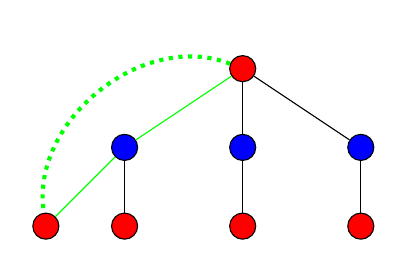
\begin{tikzpicture}[every node/.style={circle, draw}]
    \node[fill=red] (root) at (0,0) {};
    \node[fill=blue] (a) at (-1.5,-1) {};
    \node[fill=blue] (b) at (0,-1) {};
    \node[fill=blue] (c) at (1.5,-1) {};
    \node[fill=red] (d) at (-2.5,-2) {};
    \node[fill=red] (e) at (-1.5,-2) {};
    \node[fill=red] (f) at (0,-2) {};
    \node[fill=red] (g) at (1.5,-2) {};
    
    \draw[green] (root) -- (a);
    \draw (root) -- (b);
    \draw (root) -- (c);
    \draw[green] (a) -- (d);
    \draw (a) -- (e);
    \draw (b) -- (f);
    \draw (c) -- (g);
    \draw[green,dotted, bend right=60,line width= 1.5pt] (root) to (d);
\end{tikzpicture}
\caption{Marcado en verde el ciclo de longitud impar, resultante de una backedge que une elementos de la misma paridad}
\end{figure} \\
\textbf{b)} Intuición para: si toda arista de $E(G) \setminus E(T)$ une un vértice de $V$ con otro de $W$, entonces $(V, W)$ es una bipartición de $G$ y, por lo tanto, $G$ es bipartito.

Esto vale porque es claro que en el árbol generador, toda arista del árbol une a uno de longitud par con uno de impar. Si esta propiedad también se mantiene para todas las demás aristas del grafo, se sigue que no hay conexiones entre miembros de la clase "distancia par" y "distancia impar", generándonos la bipartición.\\
\begin{figure}[h]
\centering
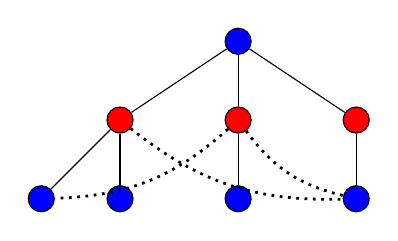
\begin{tikzpicture}[every node/.style={circle, draw}]
    \node[fill=blue] (root) at (0,0) {};
    \node[fill=red] (a) at (-1.5,-1) {};
    \node[fill=red] (b) at (0,-1) {};
    \node[fill=red] (c) at (1.5,-1) {};
    \node[fill=blue] (d) at (-2.5,-2) {};
    \node[fill=blue] (e) at (-1.5,-2) {};
    \node[fill=blue] (f) at (0,-2) {};
    \node[fill=blue] (g) at (1.5,-2) {};
    
    \draw (root) -- (a);
    \draw (root) -- (b);
    \draw (root) -- (c);
    \draw (a) -- (d);
    \draw (a) -- (e);
    \draw (b) -- (f);
    \draw (c) -- (g);
    
    \draw[dotted, bend right=20,line width = 1pt] (b) to (g);
    \draw[dotted, bend left=20,line width = 1pt] (b) to (d);
    \draw[dotted, bend right=20,line width = 1pt] (a) to (g);
\end{tikzpicture}
\caption{Se observa que como las unicas backedges que existen en G no vinculan miembros de la misma paridad en T, por lo tanto el coloreo define biparticiones}
\end{figure}
\end{document}
